%!TEX TS-program = Arara
% arara: pdflatex: {shell: yes}
\documentclass[14pt,ngerman]{beamer}

\usepackage[T1]{fontenc}
\usepackage{booktabs}
\usepackage{babel}
\usepackage{graphicx}
\usepackage{csquotes}


\usepackage{listofitems}
\setsepchar{;}

\usepackage{xcolor}
\usepackage{tikz}
\usetikzlibrary{shapes}
\usetikzlibrary{shadows}
\usetikzlibrary{positioning}
\usetikzlibrary{calc}
\usepackage{calc,tikzlings}
\usepackage{listings}
\usepackage{bera}
 
\definecolor{colBack}{rgb}{1,1,0.8}
\definecolor{hellgelb}{rgb}{1,1,0.8}
\definecolor{colKeys}{rgb}{0,0,1}
\definecolor{colIdentifier}{rgb}{0,0,0}
\definecolor{colComments}{rgb}{1,0,0}
\definecolor{colString}{rgb}{0,0.5,0}
 
\lstset{%
    float=hbp,%
    basicstyle=\ttfamily\footnotesize, %
    identifierstyle=\color{colIdentifier}, %
    keywordstyle=\color{colKeys}, %
    stringstyle=\color{colString}, %
    commentstyle=\color{colComments}, %
    columns=flexible, %
    tabsize=2, %
    frame=single, %
    extendedchars=true, %
    showspaces=false, %
    showstringspaces=false, %
    numbers=left, %
    numberstyle=\tiny, %
    breaklines=true, %
    backgroundcolor=\color{colBack}, %
    breakautoindent=true, %
    captionpos=b,
    language={[LaTeX]TeX},
    morekeywords={draw,node,node,coordinate,grid,rounded,thick, corners,very,minimum,fill,width,height,rectangle,step,thin,readlist,foreachitem,setsepchar}
}

\lstset{literate=%
    {Ö}{{\"O}}1
    {Ä}{{\"A}}1
    {Ü}{{\"U}}1
    {ß}{{\ss}}1
    {ü}{{\"u}}1
    {ä}{{\"a}}1
    {ö}{{\"o}}1
    {~}{{\textasciitilde}}1
}

\author{Uwe Ziegenhagen}
\title{\textit{TikZ}ische Erlebnisse}
\subtitle{Dante Frühjahrstagung 2025}


\begin{document}

\begin{frame}

\maketitle

\end{frame}

\begin{frame}
\frametitle{Inhalt}

\begin{itemize}
\item Kurze (nicht vollständige) Vorstellung \newline von TikZ-Grundlagen
\item Beispiele, Beispiele, Beispiele\ldots 
\item Siehe auch \url{https://github.com/UweZiegenhagen/TikZ_Tutorial}
\end{itemize}

\end{frame}

\section{Geschichte und Grundlagen} 

\begin{frame}
\frametitle{Geschichte}

\begin{itemize}
\item TikZ = \enquote{TikZ ist kein Zeichenprogramm}
\item TikZ = \enquote{Frontend} für PGF (\enquote{portable graphics format})
\item Entwickler Till Tantau, Christian Feuersänger
\item Erscheinungsjahr 2005
\end{itemize}
\end{frame}


\begin{frame}[containsverbatim]
\frametitle{Einfache Linien}

\begin{lstlisting}
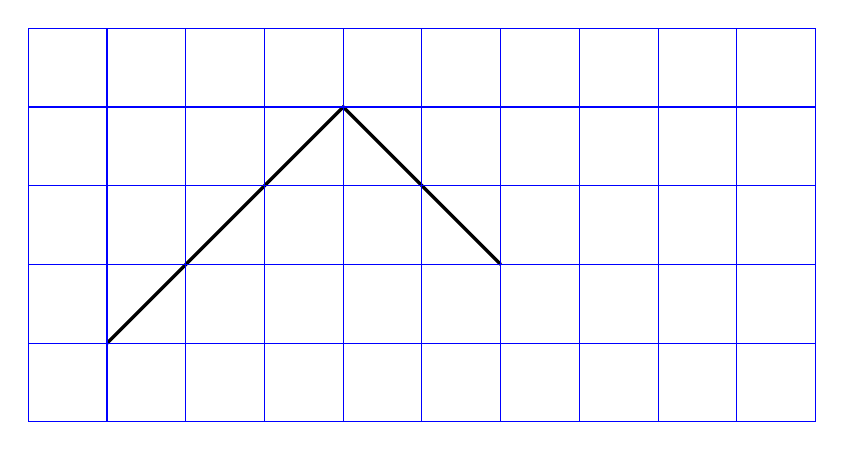
\begin{tikzpicture}
\draw[very thick] (1,1) -- (4,4) -- (6,2);
\draw[step=1cm,blue,thin] (0,0) grid (10,5);
\end{tikzpicture}
\end{lstlisting}

\begin{center}
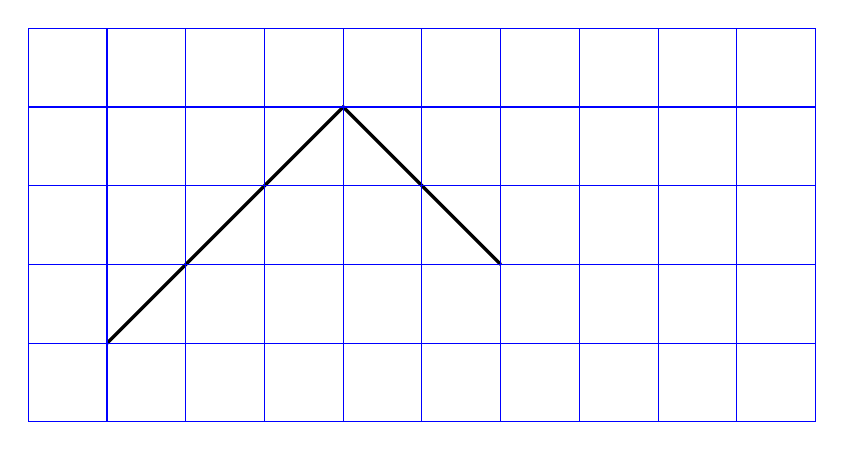
\begin{tikzpicture}
\draw[very thick] (1,1) -- (4,4) -- (6,2);
\draw[step=1cm,blue,thin] (0,0) grid (10,5);
\end{tikzpicture}
\end{center}


\end{frame}



\begin{frame}[containsverbatim]
\frametitle{Liniendicken}

\begin{lstlisting}

\begin{tikzpicture}
\draw[ultra thin] (2,1) -- (2,3);
\draw[very thin] (2.5,1) -- (2.5,3);
\draw[thin] (3,1) -- (3,3);
\draw[semithick] (3.5,1) -- (3.5,3);
\draw[thick] (4,1) -- (4,3);
\draw[very thick] (4.5,1) -- (4.5,3);
\draw[ultra thick] (5,1) -- (5,3);
\draw[line width=4pt] (5.5,1) -- (5.5,3);
\end{tikzpicture}
\end{lstlisting}

\begin{center}

\begin{tikzpicture}
\draw[ultra thin] (2,1) -- (2,3);
\draw[very thin] (2.5,1) -- (2.5,3);
\draw[thin] (3,1) -- (3,3);
\draw[semithick] (3.5,1) -- (3.5,3);
\draw[thick] (4,1) -- (4,3);
\draw[very thick] (4.5,1) -- (4.5,3);
\draw[ultra thick] (5,1) -- (5,3);
\draw[line width=4pt] (5.5,1) -- (5.5,3);
\end{tikzpicture}
\end{center}


\end{frame}

\begin{frame}[containsverbatim]
\frametitle{Linienstile}

\begin{lstlisting}
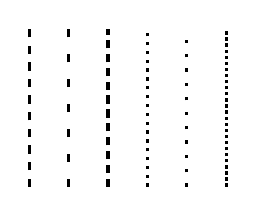
\begin{tikzpicture}
\draw[very thick, dashed] (2,1) -- (2,3);
\draw[very thick, loosely dashed] (2.5,1) -- (2.5,3);
\draw[very thick, densely dashed] (3,1) -- (3,3);
\draw[very thick, dotted] (3.5,1) -- (3.5,3);
\draw[very thick, loosely dotted] (4,1) -- (4,3);
\draw[very thick, densely dotted] (4.5,1) -- (4.5,3);
\end{tikzpicture}
\end{lstlisting}


\begin{center}
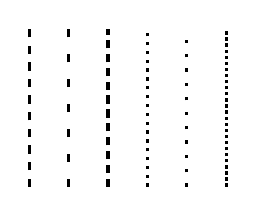
\begin{tikzpicture}
\draw[very thick, dashed] (2,1) -- (2,3);
\draw[very thick, loosely dashed] (2.5,1) -- (2.5,3);
\draw[very thick, densely dashed] (3,1) -- (3,3);
\draw[very thick, dotted] (3.5,1) -- (3.5,3);
\draw[very thick, loosely dotted] (4,1) -- (4,3);
\draw[very thick, densely dotted] (4.5,1) -- (4.5,3);
\end{tikzpicture}
\end{center}


\end{frame}



\begin{frame}[containsverbatim]
\frametitle{Rel. Koordinaten I}

mit Update der Koordinaten

\begin{lstlisting}[basicstyle=\ttfamily\scriptsize]
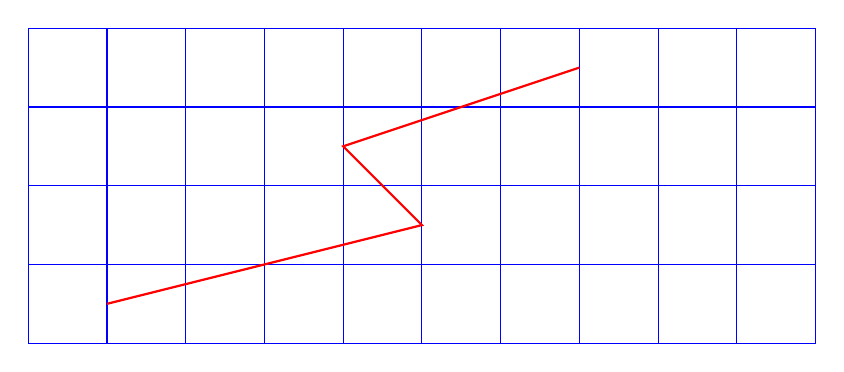
\begin{tikzpicture}
\draw[step=1cm,blue,thin] (0,0) grid (10,4);

\draw[thick, red] (1,0.5) -- ++(4,1) -- ++(-1,1) -- ++(3,1);
\end{tikzpicture}
\end{lstlisting}

\begin{center}
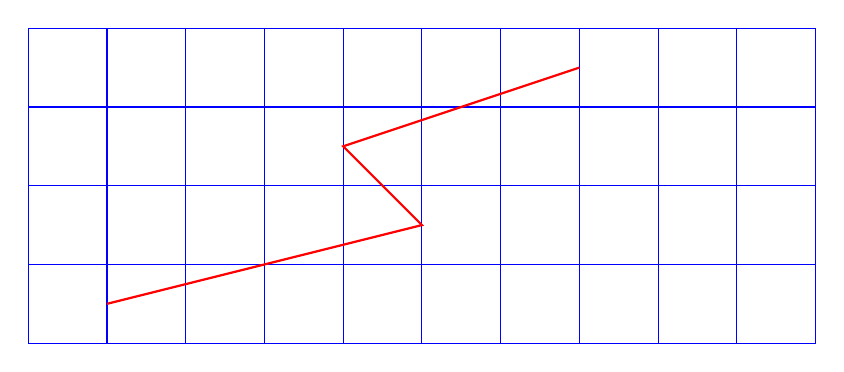
\begin{tikzpicture}
\draw[step=1cm,blue,thin] (0,0) grid (10,4);

\draw[thick, red] (1,0.5) -- ++(4,1) -- ++(-1,1) -- ++(3,1);
\end{tikzpicture}
\end{center}

\end{frame}


\begin{frame}[containsverbatim]
\frametitle{Rel. Koordinaten II}

ohne Update der Koordinaten

\begin{lstlisting}[basicstyle=\ttfamily\scriptsize]
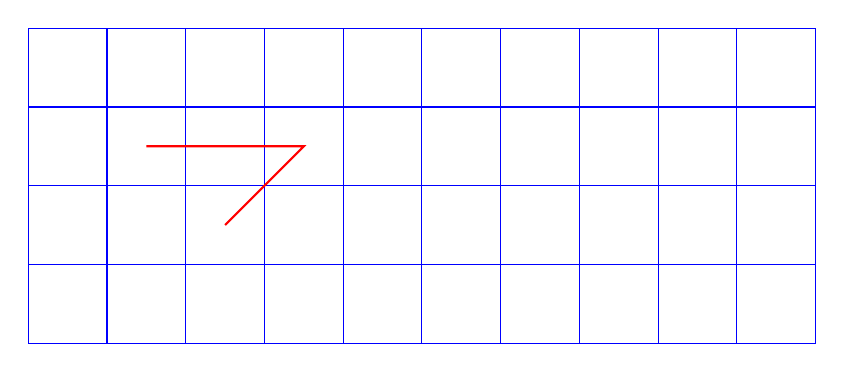
\begin{tikzpicture}
\draw[step=1cm,blue,thin] (0,0) grid (10,4);

\draw[thick, red] (2.5,1.5) -- +(1,1) -- +(-1,1);
\end{tikzpicture}
\end{lstlisting}


\begin{center}
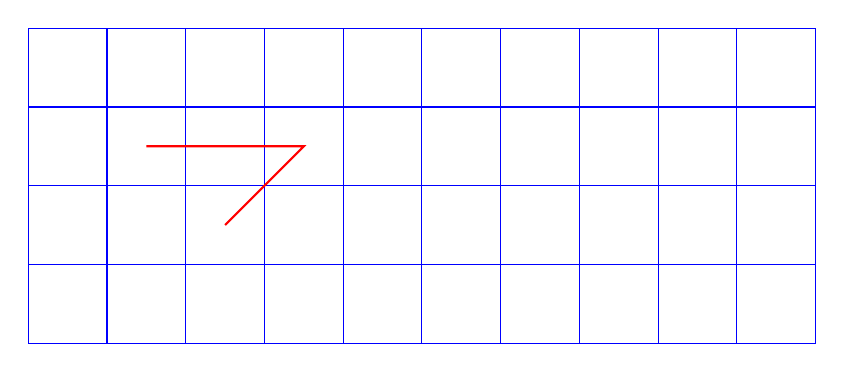
\begin{tikzpicture}
\draw[step=1cm,blue,thin] (0,0) grid (10,4);

%\draw[thick, red] (2.5,2.5) -- ++(1,1) -- ++(-1,1);

\draw[thick, red] (2.5,1.5) -- +(1,1) -- +(-1,1);
\end{tikzpicture}
\end{center}

\end{frame}


\begin{frame}[containsverbatim]
\frametitle{Nodes und Coordinates}

\begin{lstlisting}[basicstyle=\ttfamily\scriptsize]
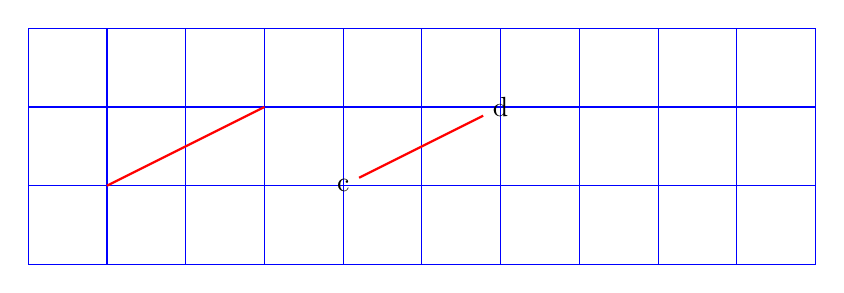
\begin{tikzpicture}
\draw[step=1cm,blue,thin] (0,0) grid (10,3);

\coordinate (a) at (1,1);
\coordinate (b) at (3,2);
\draw[red, thick] (a) -- (b);

\node (c) at (4,1){c};
\node (d) at (6,2){d};
\draw[red, thick] (c) -- (d);
\end{tikzpicture}
\end{lstlisting}

\begin{center}
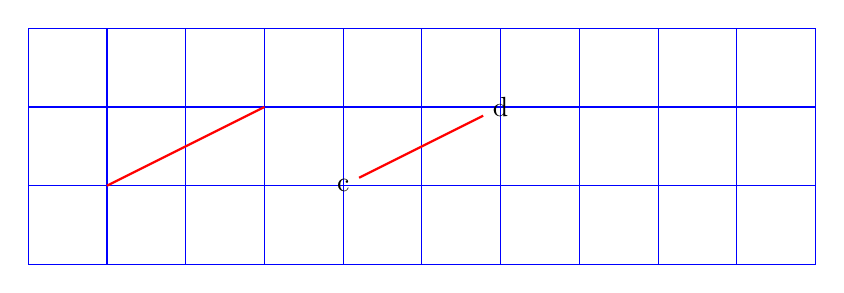
\begin{tikzpicture}
\draw[step=1cm,blue,thin] (0,0) grid (10,3);

\coordinate (a) at (1,1);
\coordinate (b) at (3,2);
\draw[red, thick] (a) -- (b);

\node (c) at (4,1){c};
\node (d) at (6,2){d};
\draw[red, thick] (c) -- (d);
\end{tikzpicture}
\end{center}

\end{frame}




\begin{frame}[containsverbatim]
\frametitle{Node Shapes}

\begin{lstlisting}[basicstyle=\ttfamily\scriptsize]
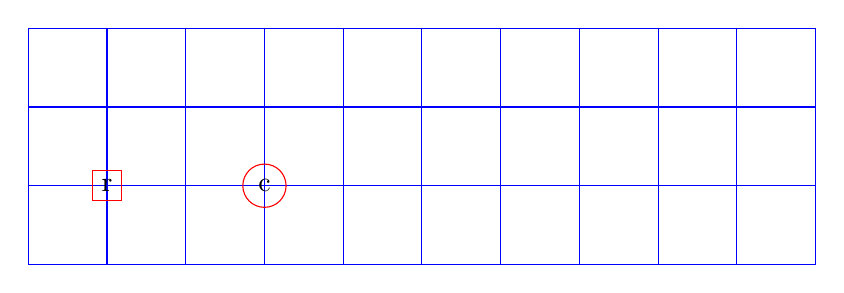
\begin{tikzpicture}
\draw[step=1cm,blue,thin] (0,0) grid (10,3);

\node[rectangle,draw = red] (r) at (1,1){r};
\node[circle,draw = red] (c) at (3,1){c};
\end{tikzpicture}
\end{lstlisting}

\begin{center}
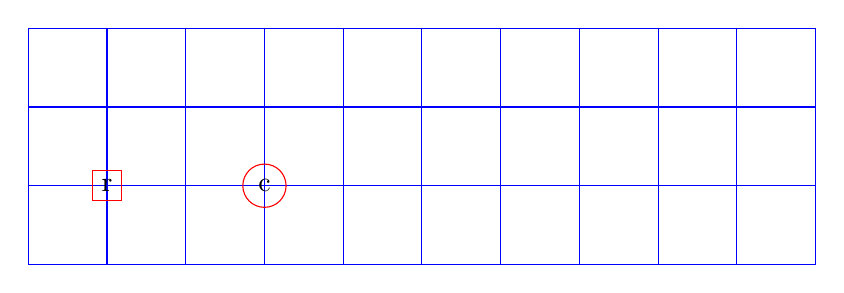
\begin{tikzpicture}
\draw[step=1cm,blue,thin] (0,0) grid (10,3);

\node[rectangle,draw = red] (r) at (1,1){r};
\node[circle,draw = red] (c) at (3,1){c};
\end{tikzpicture}
\end{center}

\begin{itemize}
	\item mehr mit \verb|\usetikzlibrary{shapes}|
\end{itemize}

\end{frame}




\begin{frame}[containsverbatim]
\frametitle{Die  \texttt{shapes} Bibliothek}

\begin{lstlisting}[basicstyle=\ttfamily\scriptsize]
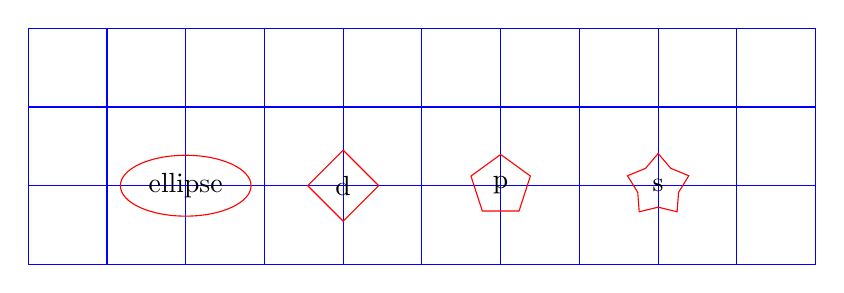
\begin{tikzpicture}
\draw[step=1cm,blue,thin] (0,0) grid (10,3);

\node[ellipse,draw = red] (e) at (2,1){ellipse};
\node[diamond,draw = red] (d) at (4,1){d};
\node[regular polygon,regular polygon sides=5,draw=red](p) at (6,1){p};
\node[star,star points=5,draw = red] (s) at (8,1){s};
\end{tikzpicture}
\end{lstlisting}

\begin{center}
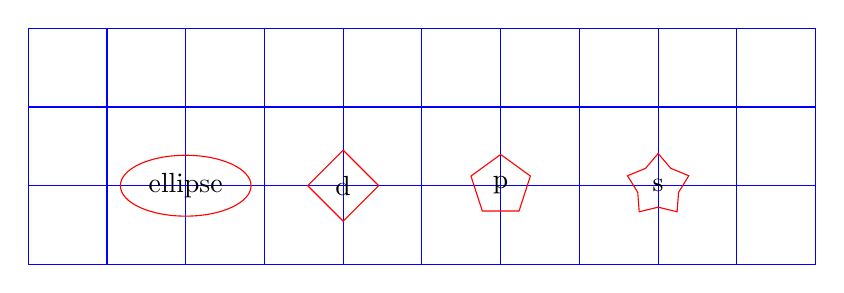
\begin{tikzpicture}
\draw[step=1cm,blue,thin] (0,0) grid (10,3);

\node[ellipse,draw = red] (e) at (2,1){ellipse};
\node[diamond,draw = red] (d) at (4,1){d};
\node[regular polygon,regular polygon sides=5,draw=red](p) at (6,1){p};
\node[star,star points=5,draw = red] (s) at (8,1){s};
\end{tikzpicture}
\end{center}

\end{frame}

\begin{frame}[containsverbatim]
\frametitle{Shapes formatieren}

\begin{lstlisting}[basicstyle=\ttfamily\scriptsize]
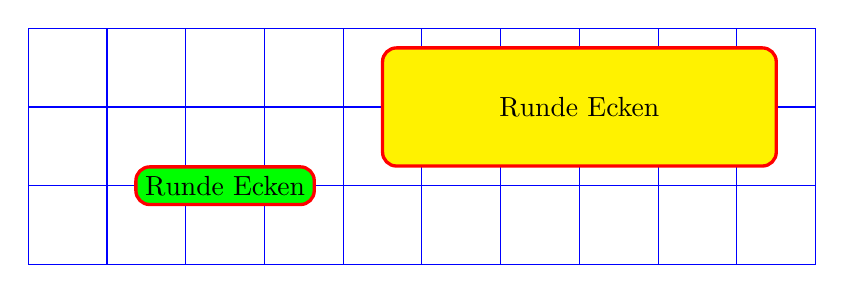
\begin{tikzpicture}
\draw[step=1cm,blue,thin] (0,0) grid (10,3);

\node[rectangle,draw = red,very thick,rounded corners=5pt,fill=green] (r) at (2.5,1){Runde Ecken};

\node[rectangle,draw = red,very thick,rounded corners=5pt,minimum width=5cm, minimum height=15mm, fill=yellow] (r) at (7,2){Runde Ecken};
\end{tikzpicture}
\end{lstlisting}

\begin{center}
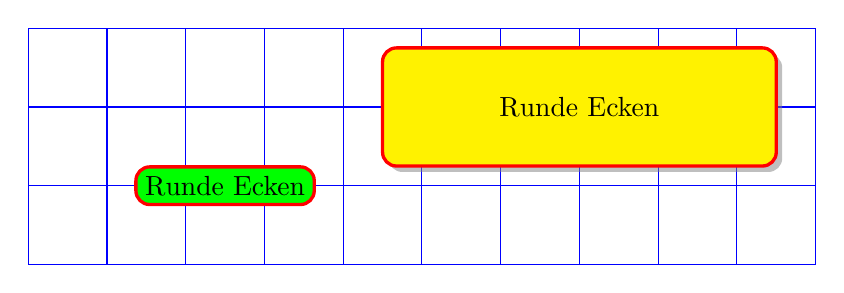
\begin{tikzpicture}
\draw[step=1cm,blue,thin] (0,0) grid (10,3);

\node[rectangle,draw = red,very thick,rounded corners=5pt,fill=green] (r) at (2.5,1){Runde Ecken};

\node[rectangle,drop shadow,draw = red,very thick,rounded corners=5pt,minimum width=5cm, minimum height=15mm, fill=yellow] (r) at (7,2){Runde Ecken};
\end{tikzpicture}
\end{center}

\end{frame}



\begin{frame}
\frametitle{Anwendungen}

\begin{itemize}
	\item Zielscheibe 10m Luftpistole
	\item Weihnachtszahlen
	\item Kalender
	\item Synthesizer-Diagramm
\end{itemize}
\end{frame}


\begin{frame}[containsverbatim]
\frametitle{Zielscheibe Luftpistole I} % [basicstyle=\ttfamily\scriptsize]

\begin{lstlisting}
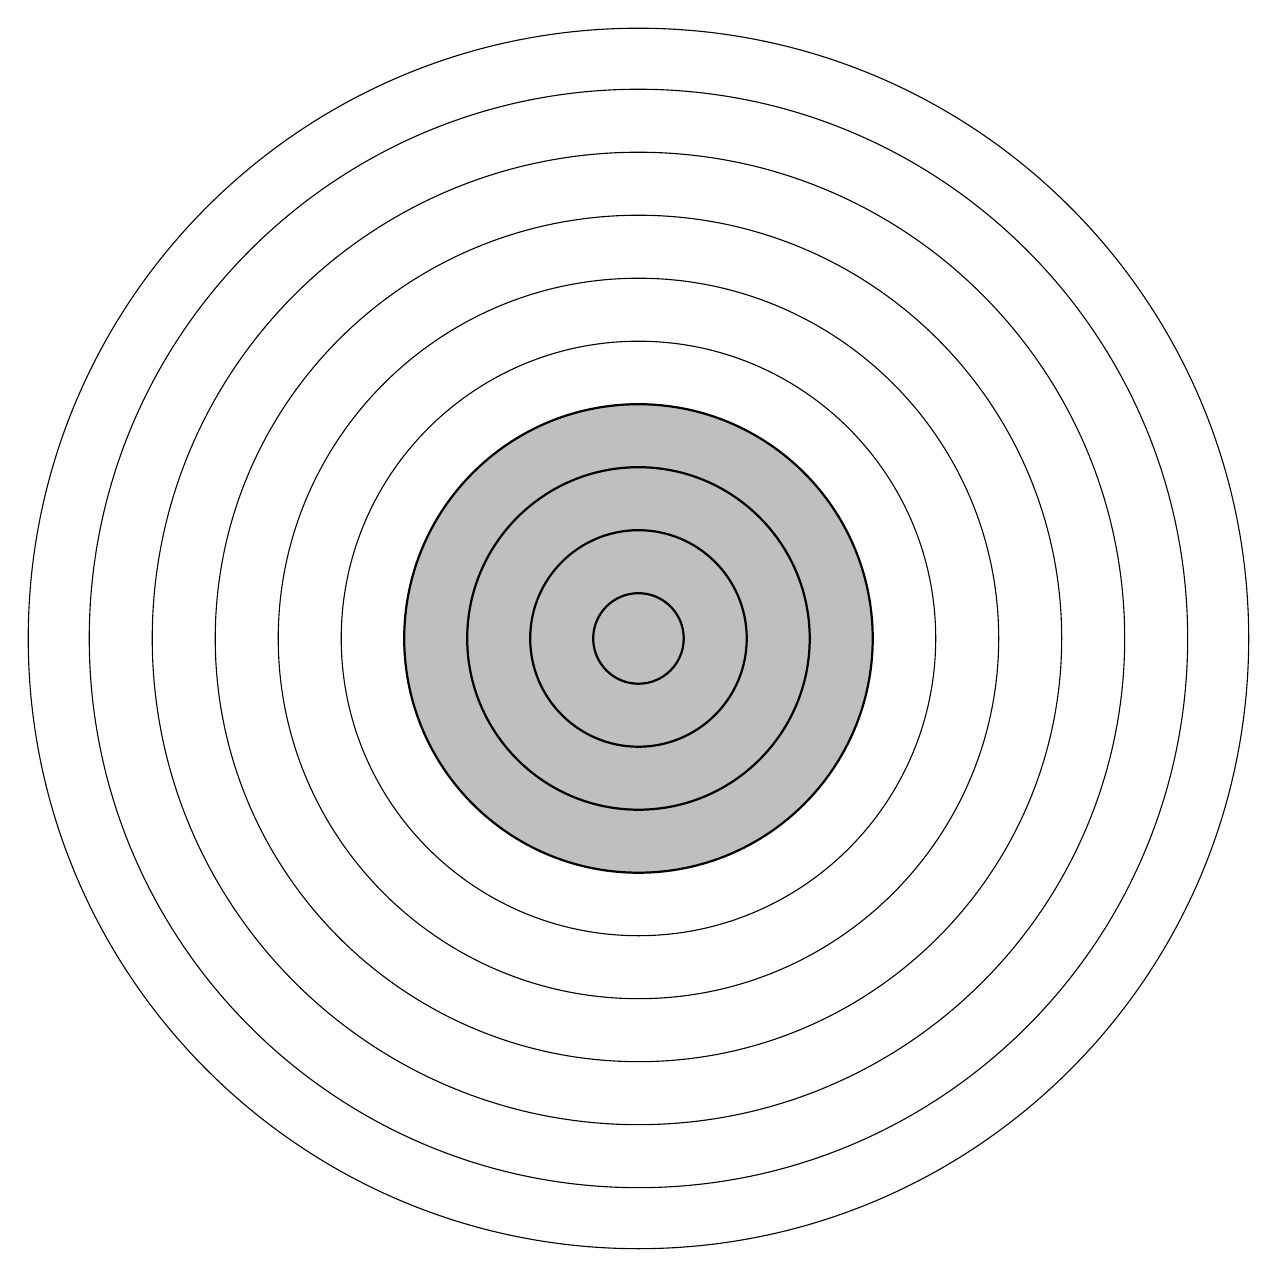
\begin{tikzpicture}
\coordinate (o) at (8,8);
\draw[black] (o) circle (77.5mm);
\draw[black] (o) circle (69.75mm);
\draw[black] (o) circle (61.75mm);
\draw[black] (o) circle (53.75mm);
\draw[black] (o) circle (45.75mm);
\draw[black] (o) circle (37.75mm);
\draw[black,thick,fill=lightgray] (o) circle (29.75mm);
\draw[black,thick] (o) circle (21.75mm);
\draw[black,thick] (o) circle (13.75mm);
\draw[black,thick] (o) circle (5.75mm);
\end{tikzpicture}
\end{lstlisting}

\end{frame}



\begin{frame}[containsverbatim]
\frametitle{Zielscheibe Luftpistole II}

\begin{center}
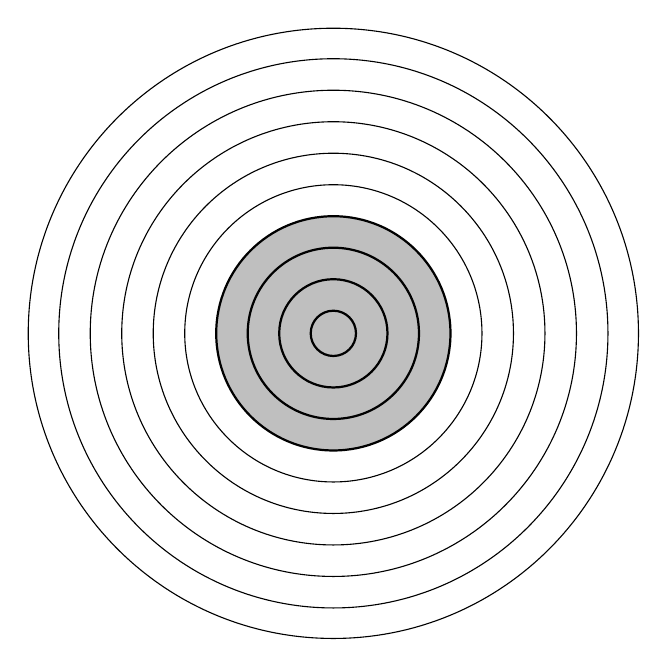
\begin{tikzpicture}[scale=0.5]
\coordinate (o) at (8,8);
\draw[black] (o) circle (77.5mm);
\draw[black] (o) circle (69.75mm);
\draw[black] (o) circle (61.75mm);
\draw[black] (o) circle (53.75mm);
\draw[black] (o) circle (45.75mm);
\draw[black] (o) circle (37.75mm);
\draw[black,thick,fill=lightgray] (o) circle (29.75mm);
\draw[black,thick] (o) circle (21.75mm);
\draw[black,thick] (o) circle (13.75mm);
\draw[black,thick] (o) circle (5.75mm);
\end{tikzpicture}
\end{center}

\end{frame}



\begin{frame}
\frametitle{Exkurs Positioning Library I}

\begin{itemize}
	\item Relative Koordinaten mit der \texttt{positioning} Library
\end{itemize}

\begin{center}
\scalebox{0.8}{%
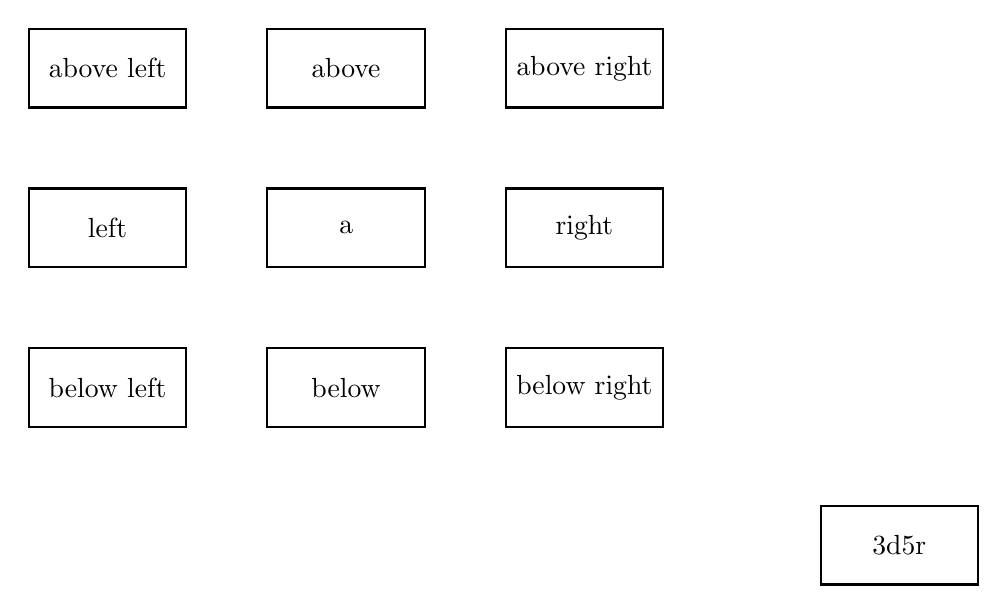
\begin{tikzpicture}[box/.style={rectangle,thick,draw=black,minimum width=20mm, minimum height=10mm,align=center}]
\node at (0,0) [box] (a) {a};
\node [below = of a,box] (b)  {below};
\node [above = of a,box] (c)  {above};
\node [left = of a,box] (d)  {left};
\node [right = of a,box] (e)  {right};
\node [below left = of a,box] (f)  {below left};
\node [below right= of a,box] (g)  {below right};
\node [above left = of a,box] (h)  {above left};
\node [above right= of a,box] (i)  {above right};
\node [below right = 3cm and 5cm of a,box] {3d5r};
\end{tikzpicture}}
\end{center}

\end{frame}


\begin{frame}[containsverbatim]
\frametitle{Exkurs Positioning Library II}

\begin{lstlisting}
\node at (0,0) [box] (a) {a};
\node [below = of a,box] (b)  {below};
\node [above = of a,box] (c)  {above};
\node [left = of a,box] (d)  {left};
\node [right = of a,box] (e)  {right};
\node [below left = of a,box] (f)  {below left};
\node [below right= of a,box] (g)  {below right};
\node [above left = of a,box] (h)  {above left};
\node [above right= of a,box] (i)  {above right};
\node [below right = 3cm and 5cm of a,box] {3d5r};
\end{lstlisting}

\end{frame}

\begin{frame}[containsverbatim]
\frametitle{Zielscheibe Luftpistole III} % [basicstyle=\ttfamily\scriptsize]

\begin{itemize}
	\item Positioning-Bibliothek laden
\end{itemize}


\begin{lstlisting}
\usetikzlibrary{positioning} 
\end{lstlisting}

\begin{lstlisting}
\begin{tikzpicture}
\node[right=0.7cm of o] {9};
\node[right=1.5cm of o] {8};
\node[right=2.3cm of o] {7};
\node[right=3.1cm of o] {6};
\node[right=3.9cm of o] {5};
\node[right=4.7cm of o] {4};
\node[right=5.5cm of o] {3};
\node[right=6.3cm of o] {2};
\node[right=7.1cm of o] {1};
\end{tikzpicture}
\end{lstlisting}\vspace*{-0.2cm}

\begin{itemize}
	\item wiederholen für left, above, below
\end{itemize}
\end{frame}

\begin{frame}[containsverbatim]
\frametitle{Zielscheibe Luftpistole IV}

\begin{center}
\resizebox{8cm}{8cm}{%
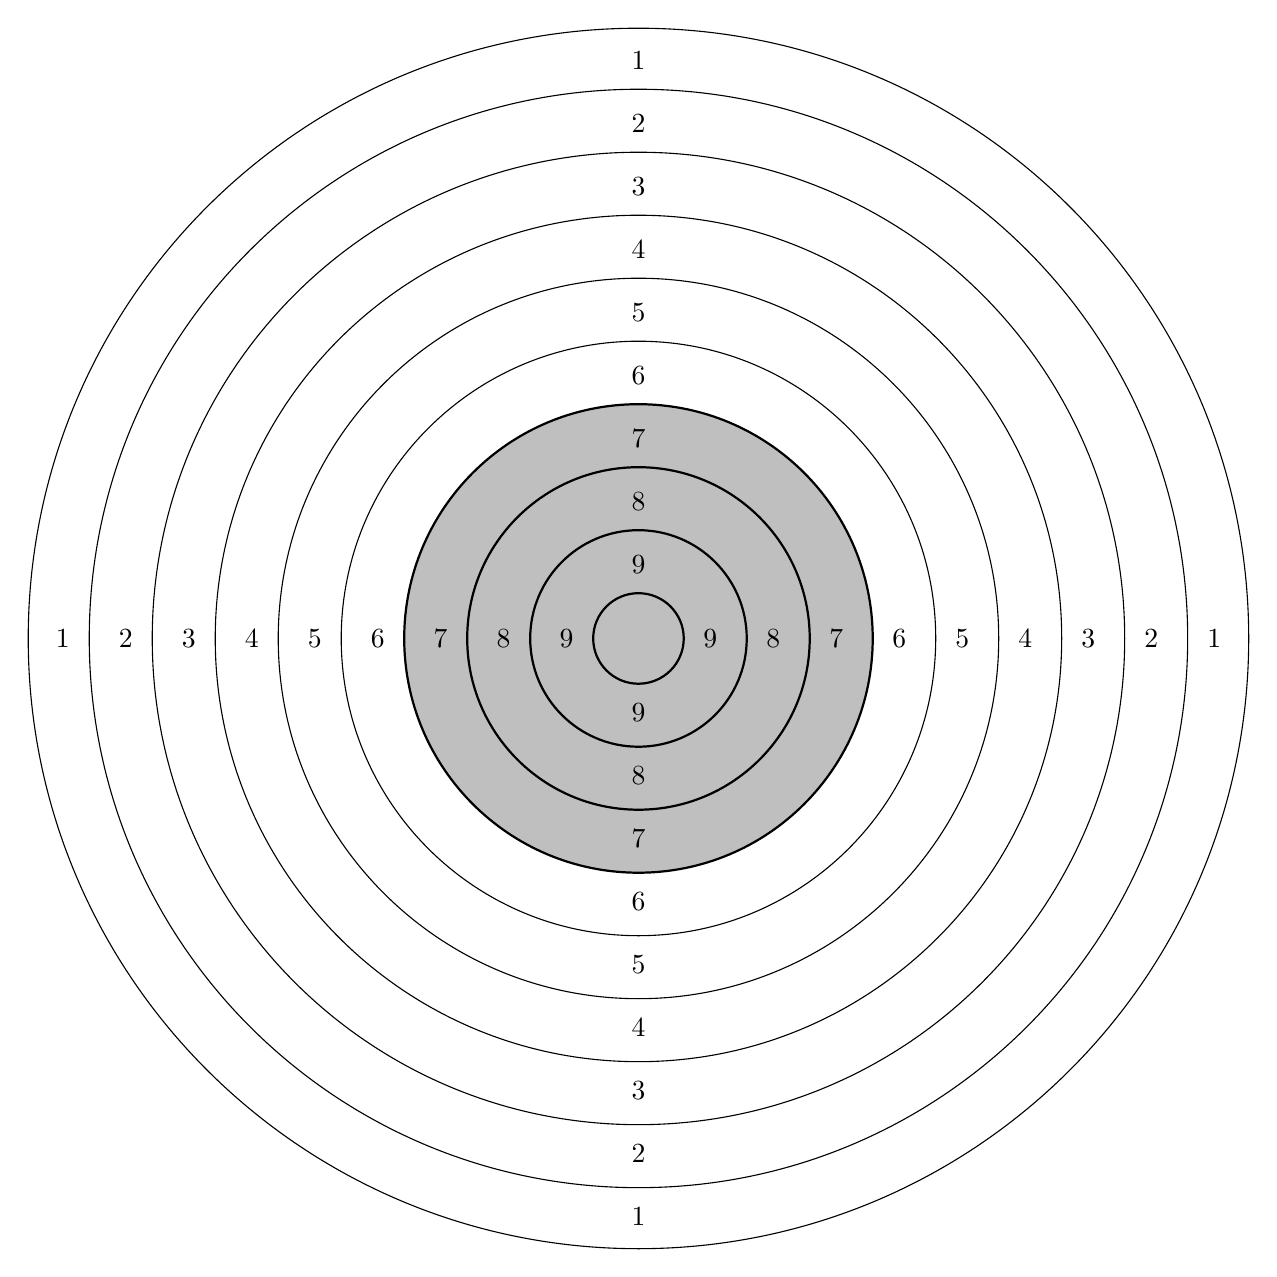
\begin{tikzpicture}
\coordinate (o) at (8,8);
\draw[black] (o) circle (77.5mm);
\draw[black] (o) circle (69.75mm);
\draw[black] (o) circle (61.75mm);
\draw[black] (o) circle (53.75mm);
\draw[black] (o) circle (45.75mm);
\draw[black] (o) circle (37.75mm);
\draw[black,thick,fill=lightgray] (o) circle (29.75mm);
\draw[black,thick] (o) circle (21.75mm);
\draw[black,thick] (o) circle (13.75mm);
\draw[black,thick] (o) circle (5.75mm);

\node[right=0.7cm of o] {9};
\node[right=1.5cm of o] {8};
\node[right=2.3cm of o] {7};
\node[right=3.1cm of o] {6};
\node[right=3.9cm of o] {5};
\node[right=4.7cm of o] {4};
\node[right=5.5cm of o] {3};
\node[right=6.3cm of o] {2};
\node[right=7.1cm of o] {1};

\node[above=0.7cm of o] {9};
\node[above=1.5cm of o] {8};
\node[above=2.3cm of o] {7};
\node[above=3.1cm of o] {6};
\node[above=3.9cm of o] {5};
\node[above=4.7cm of o] {4};
\node[above=5.5cm of o] {3};
\node[above=6.3cm of o] {2};
\node[above=7.1cm of o] {1};

\node[left=0.7cm of o] {9};
\node[left=1.5cm of o] {8};
\node[left=2.3cm of o] {7};
\node[left=3.1cm of o] {6};
\node[left=3.9cm of o] {5};
\node[left=4.7cm of o] {4};
\node[left=5.5cm of o] {3};
\node[left=6.3cm of o] {2};
\node[left=7.1cm of o] {1};


\node[below=0.7cm of o] {9};
\node[below=1.5cm of o] {8};
\node[below=2.3cm of o] {7};
\node[below=3.1cm of o] {6};
\node[below=3.9cm of o] {5};
\node[below=4.7cm of o] {4};
\node[below=5.5cm of o] {3};
\node[below=6.3cm of o] {2};
\node[below=7.1cm of o] {1};
\end{tikzpicture}}
\end{center}

\end{frame}

\begin{frame}[containsverbatim]
\frametitle{Zielscheibe Luftpistole V}

\begin{itemize}
\item Code vereinfachen mit \texttt{listofitems} Paket
\end{itemize}


\begin{lstlisting}
\usepackage{listofitems}
\setsepchar{;}
\coordinate (o) at (8,8);
\draw[black,thick,fill=lightgray] (o) circle (29.75mm);
\readlist\kreise{77.5;69.75;61.75;53.75;45.75;37.75;21.75;13.75;5.75}
\foreachitem\kreis\in\kreise{
	\draw[black] (o) circle (\kreis mm);
}
\readlist\labels{7.1;6.3;5.5;4.7;3.9;3.1;2.3;1.5;0.7}
\readlist\directions{right;above;left;below}
\foreachitem\direction\in\directions{
  \foreachitem\label\in\labels{
    \node[\direction=\label cm of o] {\labelcnt};
   }}
\end{lstlisting}

\end{frame}

\begin{frame}
\frametitle{Zielscheibe Luftpistole VI}

\begin{center}
\resizebox{8cm}{8cm}{%
\begin{tikzpicture}
\coordinate (o) at (8,8);
\draw[black,thick,fill=lightgray] (o) circle (29.75mm);
\readlist\kreise{77.5;69.75;61.75;53.75;45.75;37.75;21.75;13.75;5.75}
\foreachitem\kreis\in\kreise{
	\draw[black] (o) circle (\kreis mm);
}
\readlist\labels{7.1;6.3;5.5;4.7;3.9;3.1;2.3;1.5;0.7}
\readlist\directions{right;above;left;below}
\foreachitem\direction\in\directions{
  \foreachitem\label\in\labels{
    \node[\direction=\label cm of o] {\labelcnt};
   }}
\end{tikzpicture}}
\end{center}
\end{frame}



\begin{frame}[containsverbatim]
\frametitle{Weihnachtszahlen I}


\begin{itemize}
\item Zahlen 1--24 für Weihnachten
\item DIN A4 Blatt gut ausfüllen
\item (Manuelle) Matrix von Nodes 
\end{itemize}

\begin{lstlisting}
\node at (0,0) {1};
\node at (1,0) {2};
\node at (2,0) {3};
\node at (3,0) {4};

\node at (0,-1) {5};
\node at (1,-1) {6};
\node at (2,-1) {7};
\node at (3,-1) {8};
\end{lstlisting}
\end{frame}

\begin{frame}[containsverbatim]
\frametitle{Weihnachtszahlen II}

\begin{center}
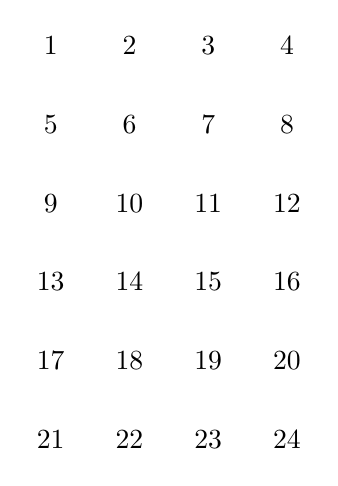
\begin{tikzpicture}
\node at (0,0) {1};
\node at (1,0) {2};
\node at (2,0) {3};
\node at (3,0) {4};

\node at (0,-1) {5};
\node at (1,-1) {6};
\node at (2,-1) {7};
\node at (3,-1) {8};

\node at (0,-2) {9};
\node at (1,-2) {10};
\node at (2,-2) {11};
\node at (3,-2) {12};

\node at (0,-3) {13};
\node at (1,-3) {14};
\node at (2,-3) {15};
\node at (3,-3) {16};

\node at (0,-4) {17};
\node at (1,-4) {18};
\node at (2,-4) {19};
\node at (3,-4) {20};

\node at (0,-5) {21};
\node at (1,-5) {22};
\node at (2,-5) {23};
\node at (3,-5) {24};
\end{tikzpicture}
\end{center}

\end{frame}

\begin{frame}[containsverbatim]
\frametitle{Weihnachtszahlen III}


\begin{lstlisting}
\tikzstyle{every node}=[circle,draw=black]

\node at (0,0) {1};
\node at (1,0) {2};
\node at (2,0) {3};
\node at (3,0) {4};

\node at (0,-1) {5};
\node at (1,-1) {6};
\node at (2,-1) {7};
\node at (3,-1) {8};
\end{lstlisting}
\end{frame}



\begin{frame}[containsverbatim]
\frametitle{Weihnachtszahlen IV}

\begin{center}
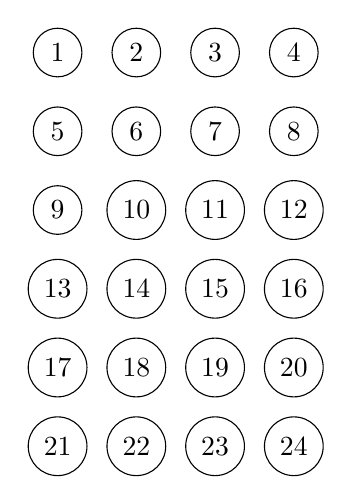
\begin{tikzpicture}
\tikzstyle{every node}=[circle,draw=black]
\node at (0,0) {1};
\node at (1,0) {2};
\node at (2,0) {3};
\node at (3,0) {4};

\node at (0,-1) {5};
\node at (1,-1) {6};
\node at (2,-1) {7};
\node at (3,-1) {8};

\node at (0,-2) {9};
\node at (1,-2) {10};
\node at (2,-2) {11};
\node at (3,-2) {12};

\node at (0,-3) {13};
\node at (1,-3) {14};
\node at (2,-3) {15};
\node at (3,-3) {16};

\node at (0,-4) {17};
\node at (1,-4) {18};
\node at (2,-4) {19};
\node at (3,-4) {20};

\node at (0,-5) {21};
\node at (1,-5) {22};
\node at (2,-5) {23};
\node at (3,-5) {24};
\end{tikzpicture}
\end{center}

\end{frame}

\begin{frame}[containsverbatim]
\frametitle{Weihnachtszahlen V}


\begin{lstlisting}
\tikzstyle{every node}=[circle,draw=black,font=\fontsize{80}{80}\selectfont,x=41mm,y=41mm,minimum width=40mm,thick]

\node at (0,0) {1};
\node at (1,0) {2};
\node at (2,0) {3};
\node at (3,0) {4};

\node at (0,-1) {5};
\node at (1,-1) {6};
\node at (2,-1) {7};
\node at (3,-1) {8};
\end{lstlisting}
\end{frame}

\begin{frame}

\begin{center}
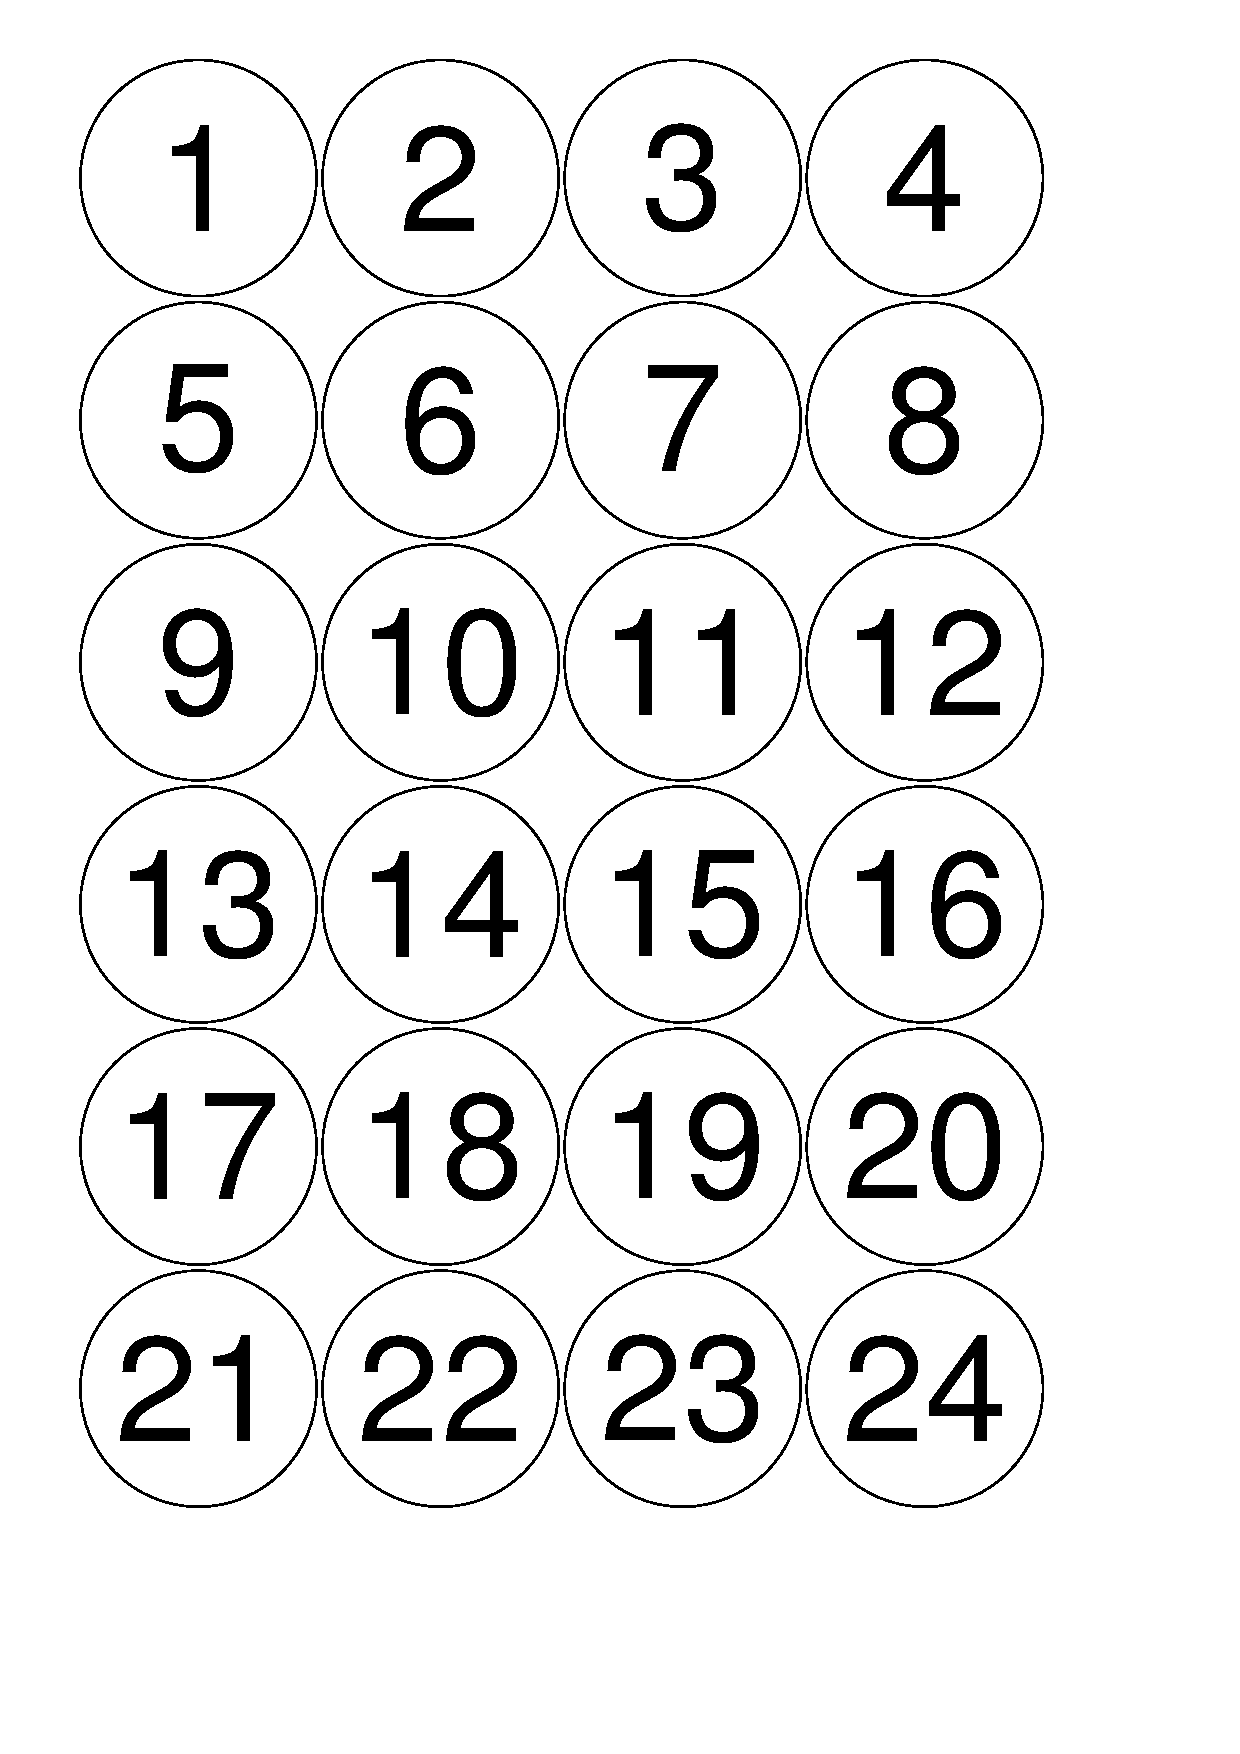
\includegraphics[width=7cm]{./Examples/Weihnachtszahlen-3}
\end{center}
\end{frame}


\begin{frame}[containsverbatim]
\frametitle{Kalender I}

\begin{itemize}
	\item Excel = Lebensnotwendigkeit für BWLer
	\item Excel nutzen, um Kalender zu \enquote{bauen}
	\item Gleiches Konzept wie bei den Weihnachtszahlen: viele Nodes
	\item Excel-Formel
\end{itemize}

\begin{lstlisting}
=WENNFEHLER("\node at (" & C$2-1 &"," & -1* $B3 & ") [" & WENN(LINKS(TEXT(DATWERT($B3&"."&C$2&"."&$B$2);"TTT");1)="S";"weekend";"workday") & "] {\hspace*{-0.9em}{"  & TEXT(DATWERT($B3&"."&C$2&"."&$B$2);"TTT")   & "}};";"")
\end{lstlisting}
\end{frame}

\begin{frame}[containsverbatim]
\frametitle{Kalender II}

\begin{itemize}
	\item \lstinline|\node at (0,-1) [workday] {\hspace*{-0.9em}{Mi}};|
\end{itemize}\vspace*{-0.5cm}

\begin{center}
\fbox{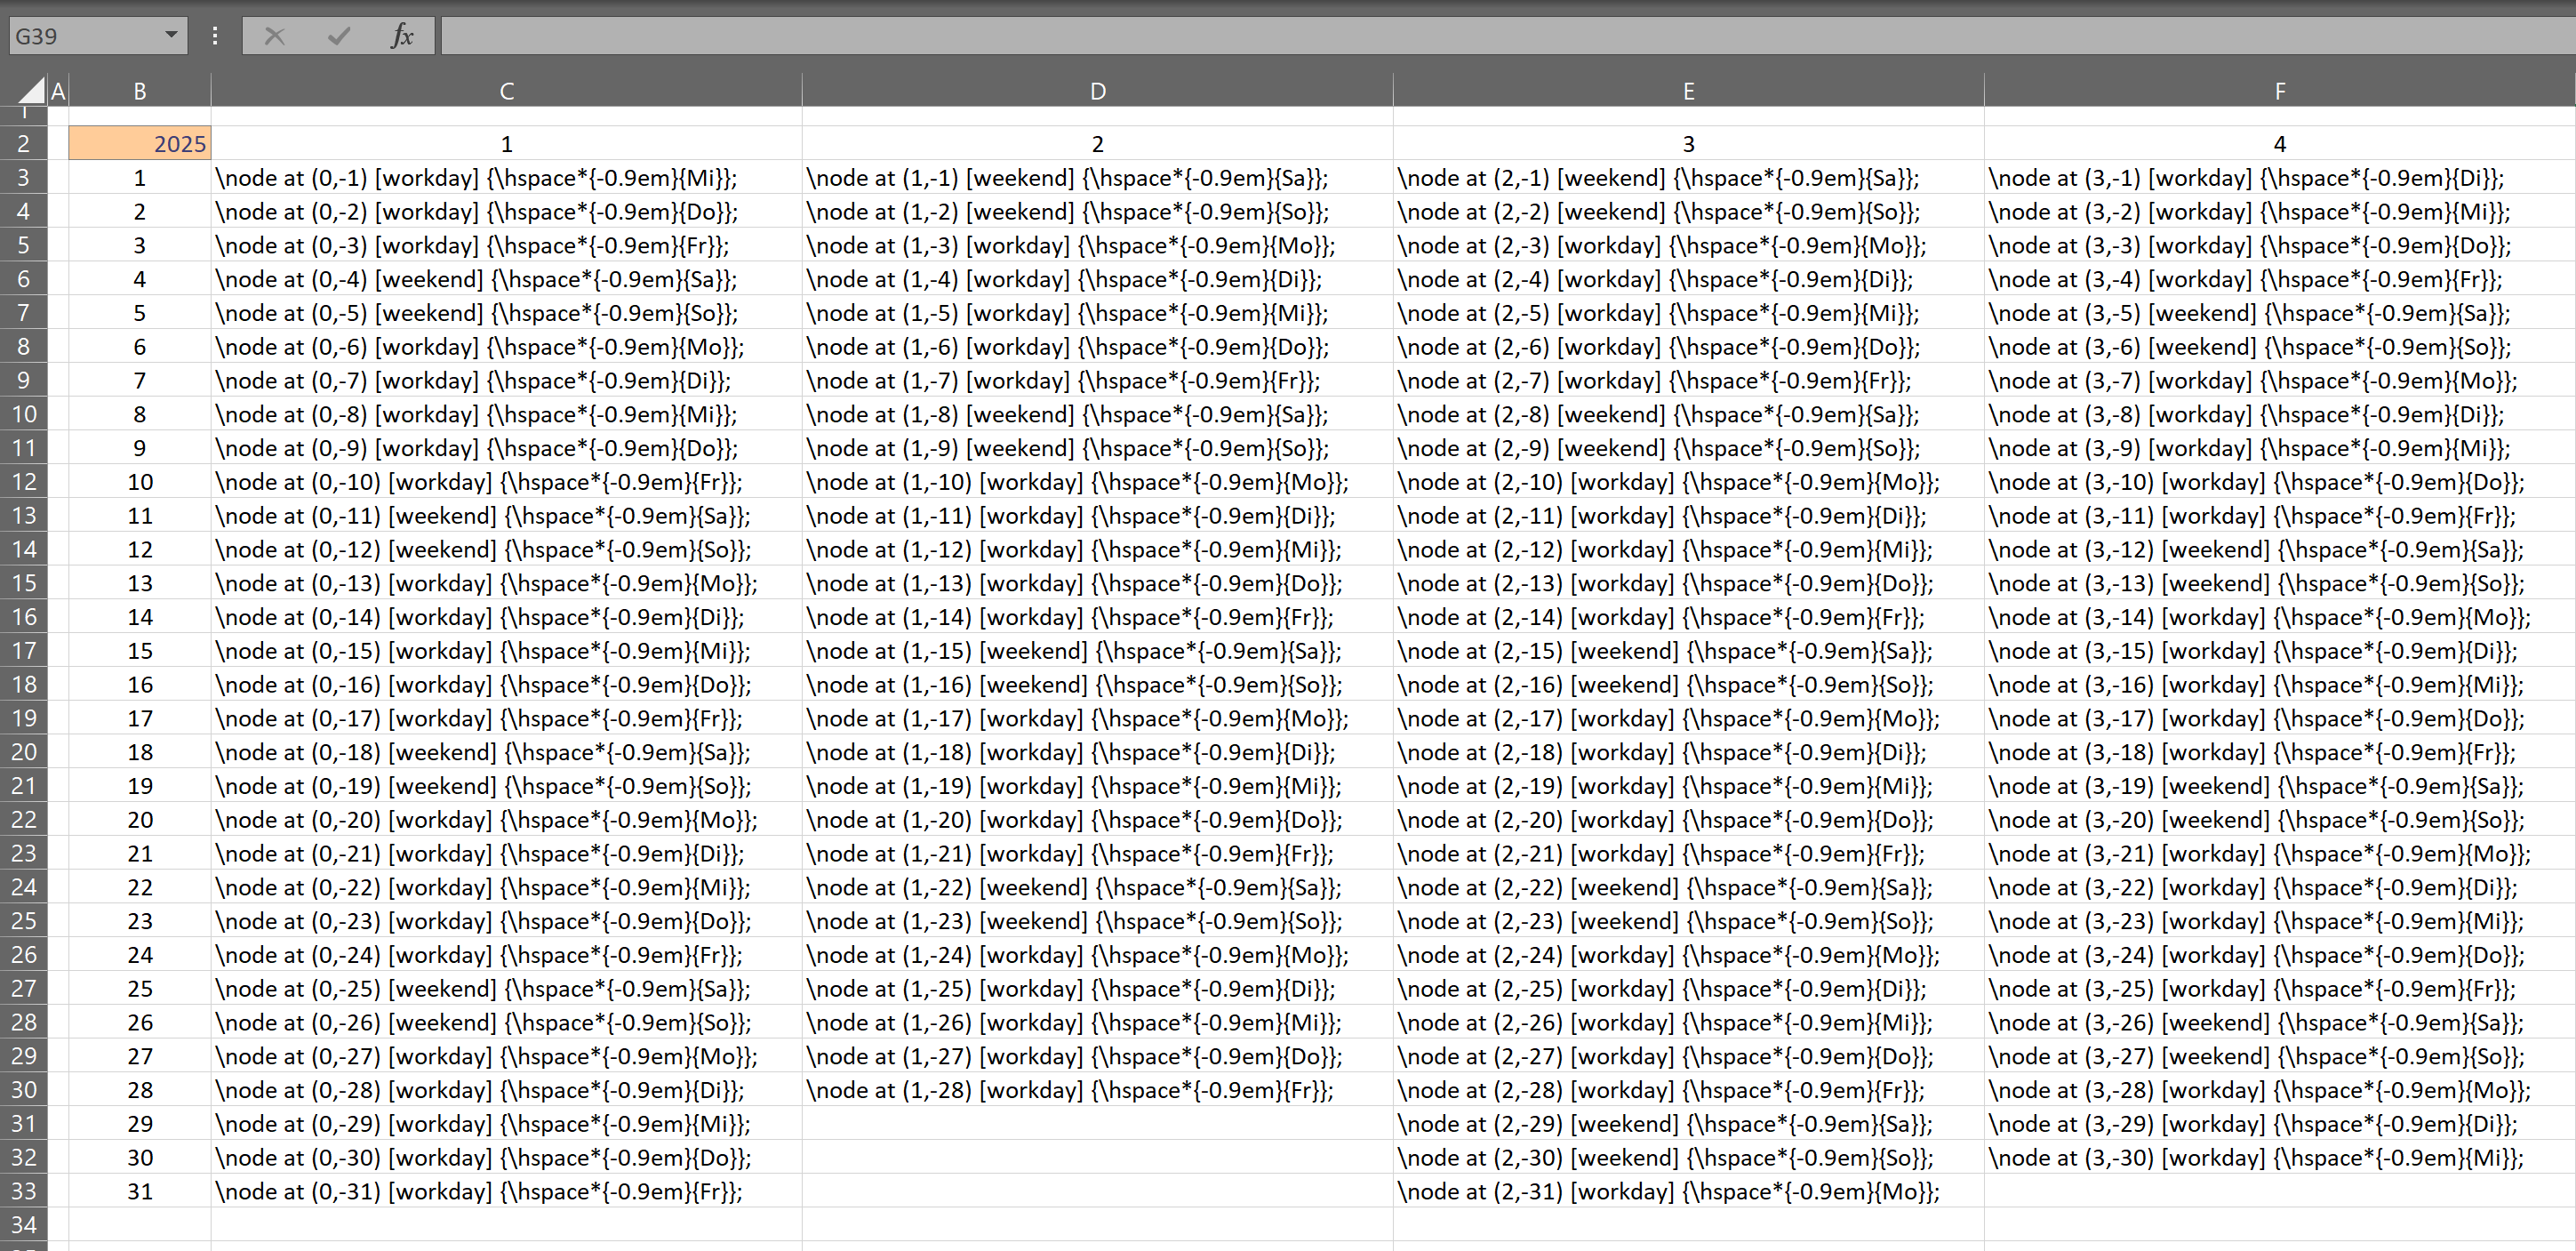
\includegraphics[width=1\textwidth]{./Examples/Kalendermacher_blog_Excel}}
\end{center}
\end{frame}


\begin{frame}[containsverbatim]
\frametitle{Kalender III}

\begin{center}
\fbox{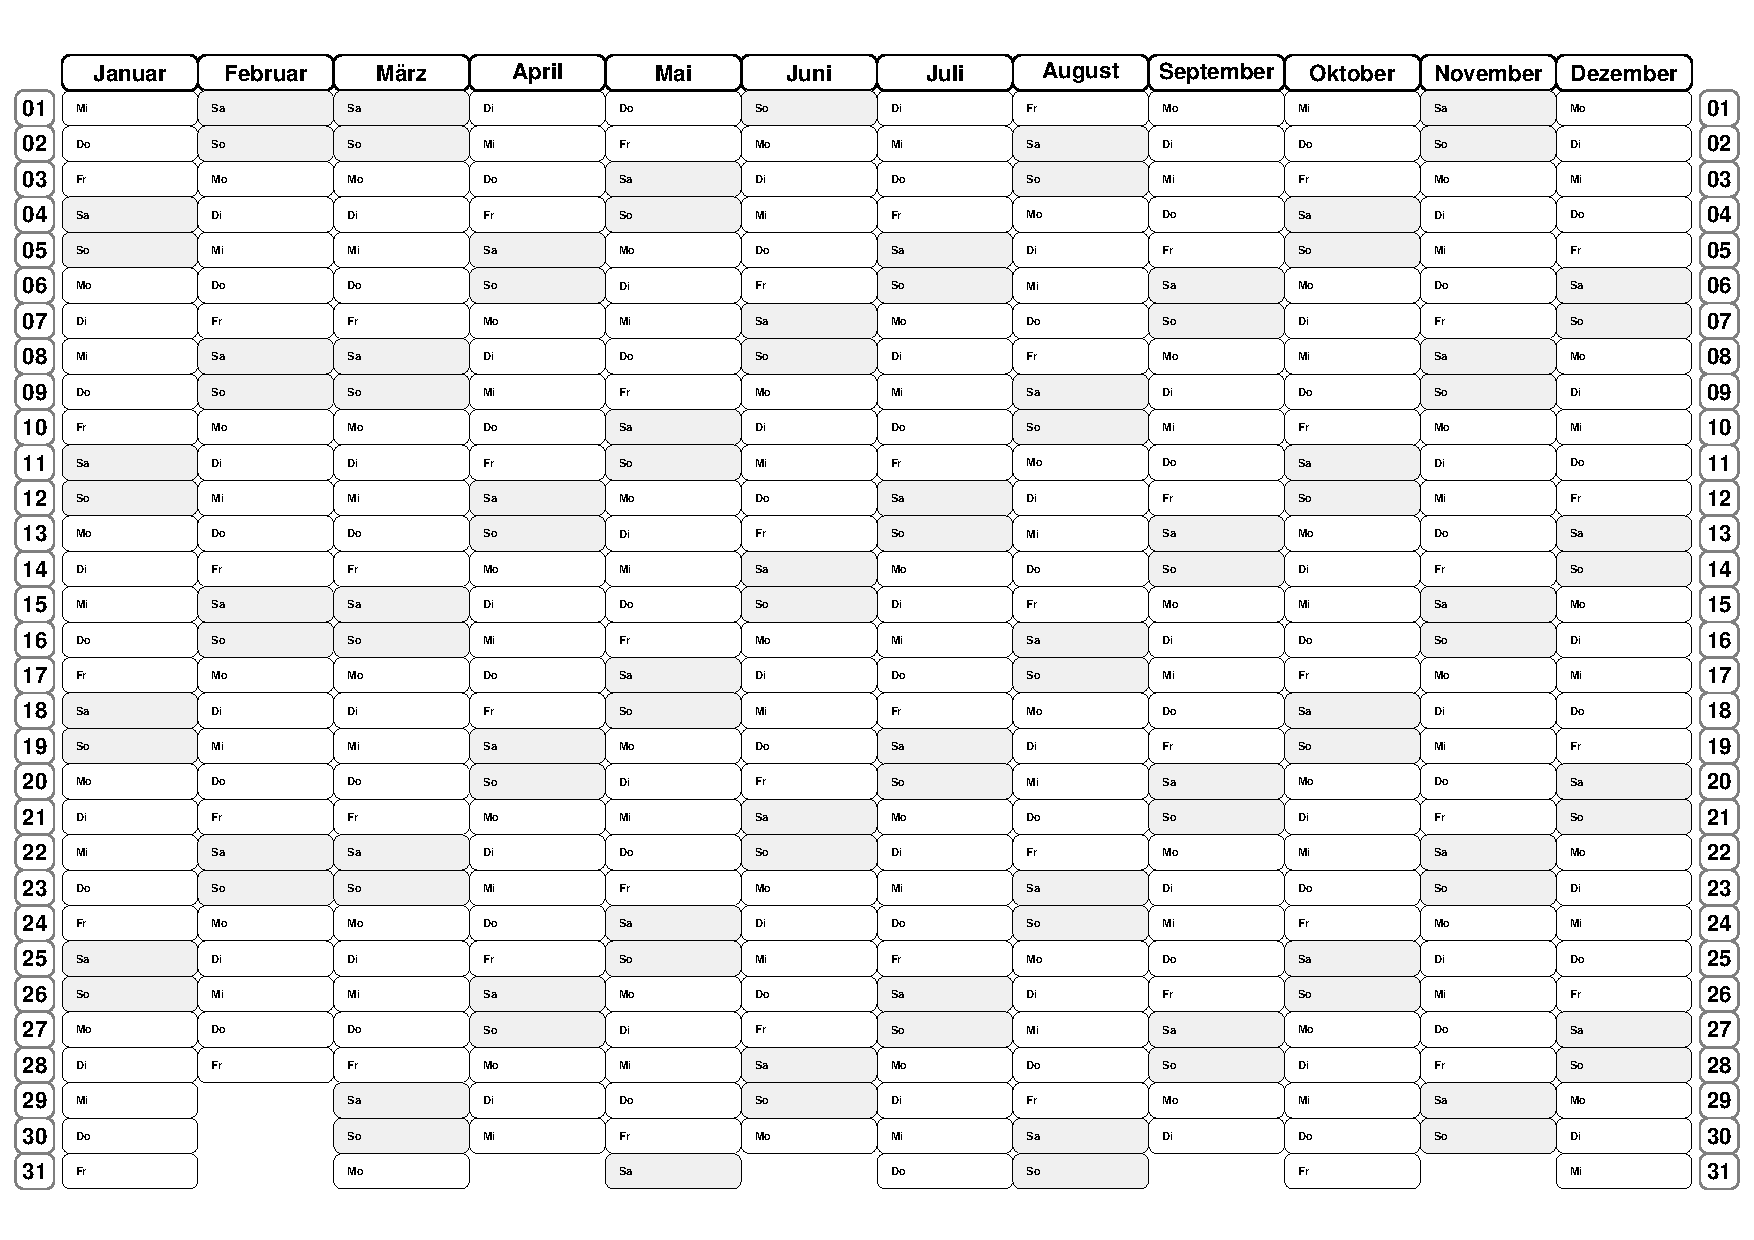
\includegraphics[width=0.95\textwidth]{./Examples/Kalender-2025}}
\end{center}
\end{frame}

\begin{frame}
\frametitle{Synthesizer-Diagramm I}

\begin{itemize}
	\item Bisher mein komplexestes TikZ-Diagramm
	\item Beschreibt den Signalweg in Synthesizer
	\item Steile Lernkurve!
\end{itemize}\vspace*{-0.5cm}

\begin{center}
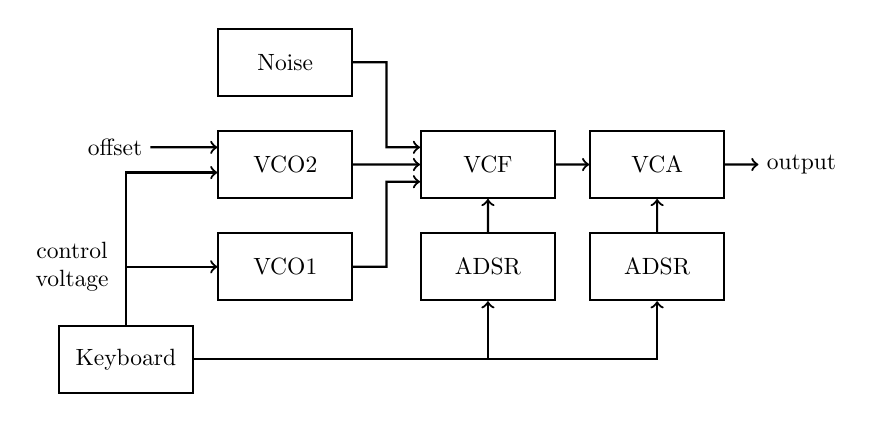
\begin{tikzpicture}[box/.style={rectangle,thick,draw=black,
minimum width=20mm, minimum height=10mm,
align=center,node distance=0.5cm},scale=0.85, transform shape]

\node at (0,0) [box] (noise) {Noise};
\node [box, below = of noise] (vco2) {VCO2};
\node [box, below = of vco2] (vco1) {VCO1};
\node [box, right = 1cm of vco2] (vcf) {VCF};
\draw [thick,->] (vco2) -- (vcf);

\coordinate (coordoffset) at ($(vco2.west)!0.5!(vco2.north west)$);

\node [left = of coordoffset](offset) {offset};
\draw [thick,->] (offset) -- (coordoffset);

\node [right = 1cm of noise] (temp1) {};

\coordinate (vcf1) at ($(vcf.west)!0.5!(vcf.north west)$);
\coordinate (vcf2) at ($(vcf.west)!0.5!(vcf.south west)$);
\coordinate (vco21) at ($(vco2.north east)!0.5!(vco2.east)$);
\coordinate (vco22) at ($(vco2.south east)!0.5!(vco2.east)$);

\node [box, right = of vcf] (vca) {VCA};
\node [box, below = of vcf] (adsr1) {ADSR};
\node [box, below = of vca] (adsr2) {ADSR};

\node [right = 0.5cm of vca] (output) {output};
\node [box, below left = 0.5cm of vco1] (keyboard) {Keyboard};

\node [left = 1.5cm of vco1,align=center](cv) {control \\ voltage };

\coordinate (noisetemp1) at ($(noise.east)!0.5!(temp1.west)$);
\coordinate (vco1adsr1) at ($(vco1.east)!0.5!(adsr1.west)$);

\coordinate (vco2vcf1) at ($(vco21)!0.5!(vcf1)$);
\coordinate (vco2vcf2) at ($(vco22)!0.5!(vcf2)$);

\draw[->,thick] (vco1.east) -- (vco1adsr1) --  (vco2vcf2) -- (vcf2);
\draw[->,thick] (noise.east) -- (noisetemp1) --  (vco2vcf1) -- (vcf1);

\draw[->,thick] (adsr1) -- (vcf);
\draw[->,thick] (adsr2) -- (vca);
\draw[->,thick] (vcf) -- (vca);
\draw[->,thick] (vca) -- (output);

\draw [thick,->] (keyboard) -| (adsr1);
\draw [thick,->] (keyboard) -| (adsr2);
\draw [thick,->] (keyboard) |- (vco1);
\draw [thick,->] (keyboard) |- (vco2.base west);
\end{tikzpicture}
\end{center}

\end{frame}

\begin{frame}
\frametitle{Synthesizer-Diagramm II}

\begin{itemize}
	\item Nodes mit absoluten Koordinaten
\item Besser mit relativen Koordinaten arbeiten!
\end{itemize}

\begin{center}
\scalebox{0.8}{%
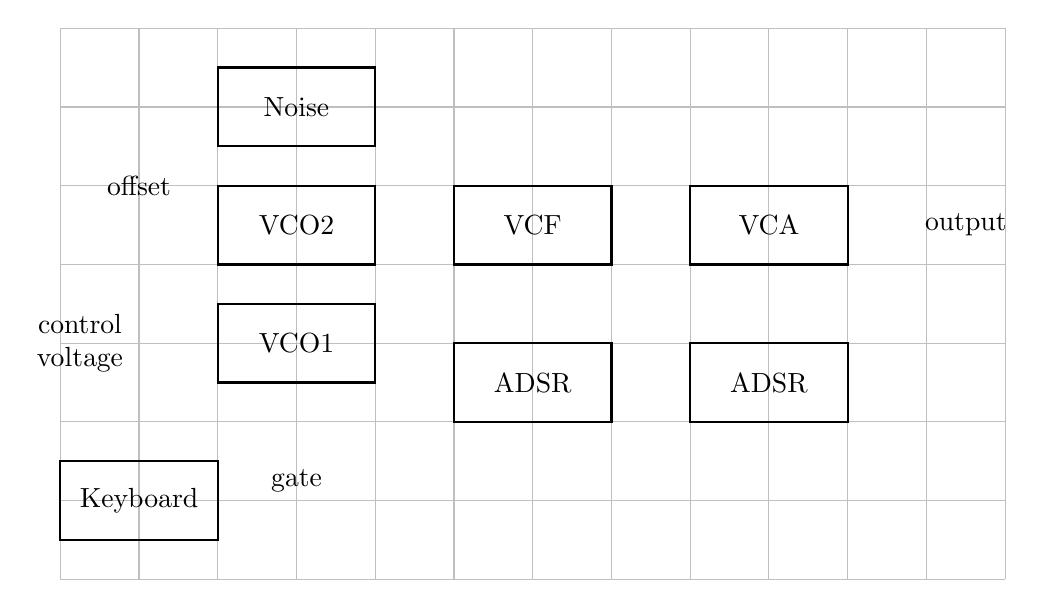
\begin{tikzpicture}[
box/.style={rectangle,thick,draw=black,minimum width=20mm, minimum height=10mm,align=center}]
\draw[step=1cm,lightgray,thin] (-1,0) grid (11,7);
\node at (2,6) [box] (noise) {Noise};
\node at (2,4.5) [box] (vco2)  {VCO2};
\node at (2,3) [box] (vco1) {VCO1};
\node at (5,4.5) [box]  (vcf) {VCF};
\node at (8,4.5) [box] (vca) {VCA};
\node at (5,2.5) [box] (adsr1) {ADSR};
\node at (8,2.5) [box] (adsr2) {ADSR};
\node at (0,1) [box] (keyboard) {Keyboard};

\node at (0,5) (offset) {offset};
\node at (10.5,4.5) (output) {output};
\node at (2,1.25) (gate) {gate};

\node [align=center] at (-0.75,3) (cv) {control \\ voltage};
\end{tikzpicture}}
\end{center}

\end{frame}



\begin{frame}
\frametitle{Synthesizer-Diagramm V}

\begin{itemize}
	\item Jeder Node hat vordefinierte Ankerpunkte
\end{itemize}

\begin{center}
\scalebox{1.15}{%
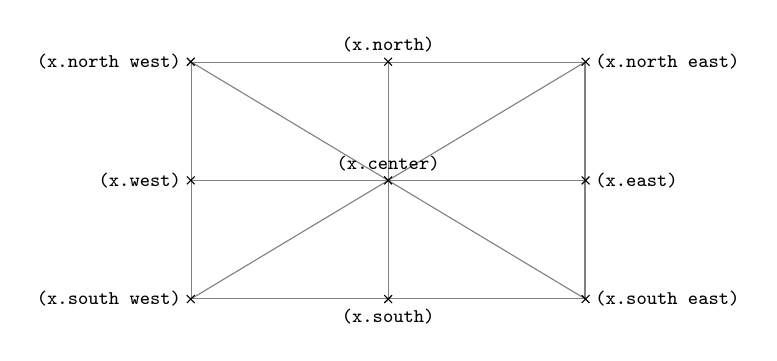
\begin{tikzpicture}[
every node/.style={font=\ttfamily\scriptsize},
mystyle/.style={gray, thin}]

\node[name=x,gray, rectangle, draw,mystyle, minimum width=5cm, minimum height=3cm] {};

\draw[mystyle]  (x.north) -- (x.south);
\draw[mystyle]  (x.east) -- (x.west);
\draw[mystyle]  (x.north east) -- (x.south west);
\draw[mystyle]  (x.south east) -- (x.north west);

\draw[] plot[mark=x] coordinates{(x.center)} node[above]{(x.center)};

\draw[] plot[mark=x] coordinates{(x.north)} node[above]{(x.north)};
\draw[] plot[mark=x] coordinates{(x.east)} node[right]{(x.east)};
\draw[] plot[mark=x] coordinates{(x.south)} node[below]{(x.south)};
\draw[] plot[mark=x] coordinates{(x.west)} node[left]{(x.west)};
\draw[] plot[mark=x] coordinates{(x.north east)} node[right]{(x.north east)};
\draw[] plot[mark=x] coordinates{(x.south east)} node[right]{(x.south east)};
\draw[] plot[mark=x] coordinates{(x.south west)} node[left]{(x.south west)};
\draw[] plot[mark=x] coordinates{(x.north west)} node[left]{(x.north west)};
\end{tikzpicture}}
\end{center}

\end{frame}

\begin{frame}
\frametitle{Synthesizer-Diagramm VI}

\begin{itemize}
	\item Pfeil von \texttt{x.north west} nach \texttt{x.south}
	\end{itemize}

\begin{center}
\scalebox{1.15}{%
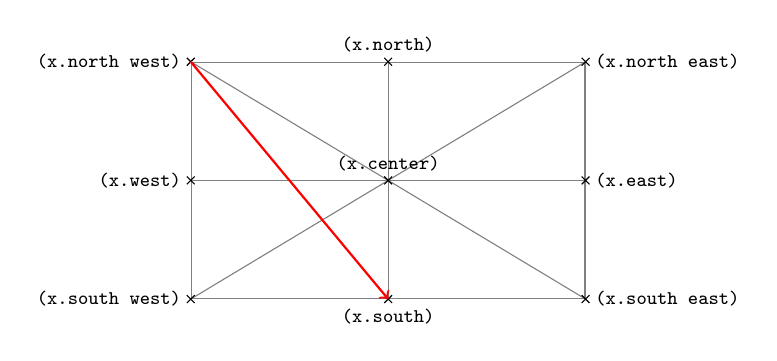
\begin{tikzpicture}[
every node/.style={font=\ttfamily\scriptsize},
mystyle/.style={gray, thin}]

\node[name=x,gray, rectangle, draw,mystyle, minimum width=5cm, minimum height=3cm] {};

\draw[mystyle]  (x.north) -- (x.south);
\draw[mystyle]  (x.east) -- (x.west);
\draw[mystyle]  (x.north east) -- (x.south west);
\draw[mystyle]  (x.south east) -- (x.north west);

\draw[] plot[mark=x] coordinates{(x.center)} node[above]{(x.center)};

\draw[] plot[mark=x] coordinates{(x.north)} node[above]{(x.north)};
\draw[] plot[mark=x] coordinates{(x.east)} node[right]{(x.east)};
\draw[] plot[mark=x] coordinates{(x.south)} node[below]{(x.south)};
\draw[] plot[mark=x] coordinates{(x.west)} node[left]{(x.west)};
\draw[] plot[mark=x] coordinates{(x.north east)} node[right]{(x.north east)};
\draw[] plot[mark=x] coordinates{(x.south east)} node[right]{(x.south east)};
\draw[] plot[mark=x] coordinates{(x.south west)} node[left]{(x.south west)};
\draw[] plot[mark=x] coordinates{(x.north west)} node[left]{(x.north west)};
\draw[->,red,thick] (x.north west) -- (x.south);
\end{tikzpicture}}
\end{center}

\end{frame}

\begin{frame}
\frametitle{Synthesizer-Diagramm VII}

\begin{itemize}
\item So weit, so gut, aber\ldots
\item Wir brauchen mehr Anker!
\end{itemize}

\begin{center}
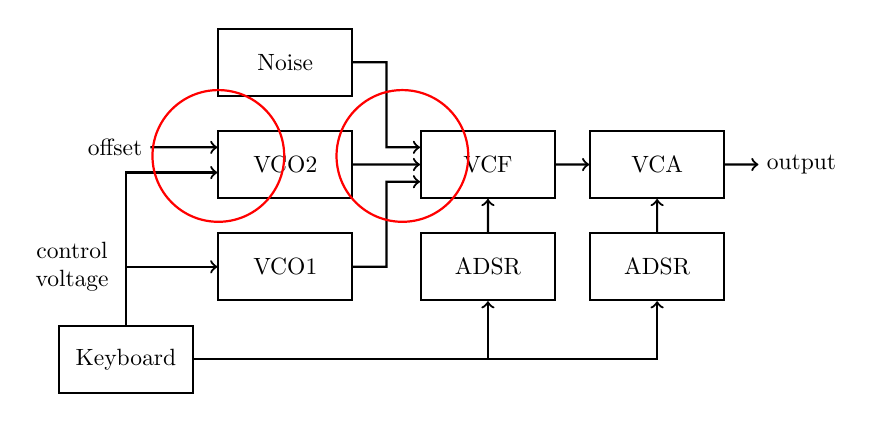
\begin{tikzpicture}[box/.style={rectangle,thick,draw=black,
minimum width=20mm, minimum height=10mm,
align=center,node distance=0.5cm},scale=0.85, transform shape]

\node at (0,0) [box] (noise) {Noise};
\node [box, below = of noise] (vco2) {VCO2};
\node [box, below = of vco2] (vco1) {VCO1};
\node [box, right = 1cm of vco2] (vcf) {VCF};
\draw [thick,->] (vco2) -- (vcf);

\coordinate (coordoffset) at ($(vco2.west)!0.5!(vco2.north west)$);

\node [left = of coordoffset](offset) {offset};
\draw [thick,->] (offset) -- (coordoffset);

\node [right = 1cm of noise] (temp1) {};

\coordinate (vcf1) at ($(vcf.west)!0.5!(vcf.north west)$);
\coordinate (vcf2) at ($(vcf.west)!0.5!(vcf.south west)$);
\coordinate (vco21) at ($(vco2.north east)!0.5!(vco2.east)$);
\coordinate (vco22) at ($(vco2.south east)!0.5!(vco2.east)$);

\node [box, right = of vcf] (vca) {VCA};
\node [box, below = of vcf] (adsr1) {ADSR};
\node [box, below = of vca] (adsr2) {ADSR};

\node [right = 0.5cm of vca] (output) {output};
\node [box, below left = 0.5cm of vco1] (keyboard) {Keyboard};

\node [left = 1.5cm of vco1,align=center](cv) {control \\ voltage };

\coordinate (noisetemp1) at ($(noise.east)!0.5!(temp1.west)$);
\coordinate (vco1adsr1) at ($(vco1.east)!0.5!(adsr1.west)$);

\coordinate (vco2vcf1) at ($(vco21)!0.5!(vcf1)$);
\coordinate (vco2vcf2) at ($(vco22)!0.5!(vcf2)$);

\draw[->,thick] (vco1.east) -- (vco1adsr1) --  (vco2vcf2) -- (vcf2);
\draw[->,thick] (noise.east) -- (noisetemp1) --  (vco2vcf1) -- (vcf1);

\draw[->,thick] (adsr1) -- (vcf);
\draw[->,thick] (adsr2) -- (vca);
\draw[->,thick] (vcf) -- (vca);
\draw[->,thick] (vca) -- (output);

\draw [thick,->] (keyboard) -| (adsr1);
\draw [thick,->] (keyboard) -| (adsr2);
\draw [thick,->] (keyboard) |- (vco1);
\draw [thick,->] (keyboard) |- (vco2.base west);

\draw [red,thick](-1,-1.4) circle (28pt);
\draw [red,thick](1.75,-1.4) circle (28pt);
\end{tikzpicture}
\end{center}

\end{frame}


\begin{frame}
\frametitle{Synthesizer-Diagramm VIII}

\begin{itemize}
	\item Zu berechnende Punkte
\end{itemize}

\begin{center}
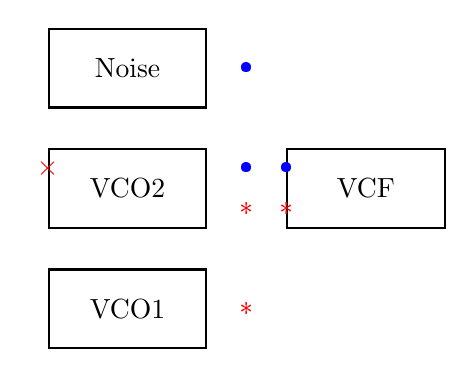
\begin{tikzpicture}[
box/.style={rectangle,thick,draw=black,
minimum width=20mm, minimum height=10mm,
align=center,node distance=0.5cm}]

\node at (0,0) [box] (noise) {Noise};
\node [box, below = of noise] (vco2) {VCO2};
\node [box, below = of vco2] (vco1) {VCO1};
\node [box, right = 1cm of vco2] (vcf) {VCF};

\coordinate (coordoffset) at ($(vco2.west)!0.5!(vco2.north west)$);
\node at (coordoffset){\textcolor{red}{$\times$}};

\node [right = 1cm of noise] (temp1) {};
\node [right = 1cm of vco1] (temp2) {};

\coordinate (vcf1) at ($(vcf.west)!0.5!(vcf.north west)$);
\coordinate (vcf2) at ($(vcf.west)!0.5!(vcf.south west)$);
\coordinate (vco21) at ($(vco2.north east)!0.5!(vco2.east)$);
\coordinate (vco22) at ($(vco2.south east)!0.5!(vco2.east)$);

\node at (vcf1){\textcolor{blue}{\textbullet}};
\node at (vcf2){\textcolor{red}{\textasteriskcentered}};

\coordinate (noisetemp1) at ($(noise.east)!0.5!(temp1.west)$);
\coordinate (vco1temp2) at ($(vco1.east)!0.5!(temp2.west)$);

\node at (noisetemp1){\textcolor{blue}{\textbullet}};
\node at (vco1temp2){\textcolor{red}{\textasteriskcentered}};

\node at (vco21){\textcolor{blue}{}};
\node at (vco22){\textcolor{blue}{}};

\coordinate (vco2vcf1) at ($(vco21)!0.5!(vcf1)$);
\coordinate (vco2vcf2) at ($(vco22)!0.5!(vcf2)$);

\node at (vco2vcf1){\textcolor{blue}{\textbullet}};
\node at (vco2vcf2){\textcolor{red}{\textasteriskcentered}};
\end{tikzpicture}
\end{center}

\end{frame}

\begin{frame}[containsverbatim]
\frametitle{Synthesizer-Diagramm IX}

\begin{itemize}
\item Koordinatenberechnungen mit der \texttt{calc} Library
\end{itemize}

\begin{lstlisting}
($<coordinate>!<number>!<coordinate>$)
\end{lstlisting}

\begin{itemize}
	\item \texttt{<coordinate>} steht dabei für eine Koordinate, die -- vielleicht etwas vereinfachend erklärt -- einfach nur ein Node ohne den (optionalen) Text ist.
	\item  \texttt{<number>} ist Zahl zwischen 0 und 1 und gibt die Prozente an, um den wir uns von Koordinate 1 zu Koordinate 2 bewegen. 
	\item  \texttt{0.25} steht also für ein Viertel des Weges 
\end{itemize}

\end{frame}

\begin{frame}[containsverbatim]
\frametitle{Synthesizer-Diagramm X}


\begin{lstlisting}
\node at (0,0) [box] (noise) {Noise};
\node [box, below = of noise] (vco2) {VCO2};
\coordinate (coordoffset) at ($(vco2.west)!0.5!(vco2.north west)$);
\node at (coordoffset){\textcolor{red}{$\times$}};

\node [left = of coordoffset](offset) {offset};
\draw [thick,->] (offset) -- (coordoffset);
\end{lstlisting}

\begin{center}
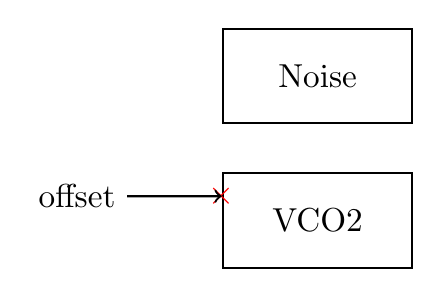
\begin{tikzpicture}[scale=1.2, transform shape,
box/.style={rectangle,thick,draw=black,
minimum width=20mm, minimum height=10mm,
align=center,node distance=0.5cm}]

\node at (0,0) [box] (noise) {Noise};
\node [box, below = of noise] (vco2) {VCO2};
\coordinate (coordoffset) at ($(vco2.west)!0.5!(vco2.north west)$);
\node at (coordoffset){\textcolor{red}{$\times$}};
\node [left = of coordoffset](offset) {offset};
\draw [thick,->] (offset) -- (coordoffset);
\end{tikzpicture}
\end{center}

\end{frame}



\begin{frame}[containsverbatim]
\frametitle{Synthesizer-Diagramm XI}

\begin{center}
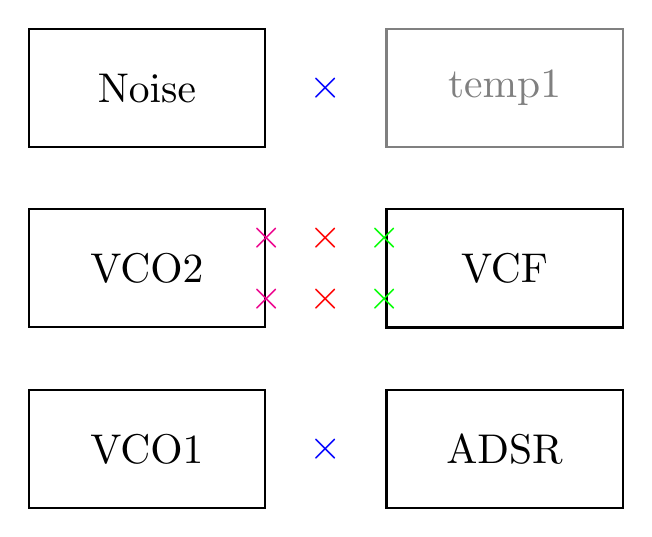
\begin{tikzpicture}[scale=1.5, transform shape,
box/.style={rectangle,thick,draw=black,
minimum width=20mm, minimum height=10mm,
align=center,node distance=0.5cm}]

\node at (0,0) [box] (noise) {Noise};
\node [box, below = of noise] (vco2) {VCO2};
\node [box, below = of vco2] (vco1) {VCO1};
\node [box, right = 1cm of vco2] (vcf) {VCF};

\node [box, gray, right = 1cm of noise] (temp1) {temp1};
\node [box, right = 1cm of vco1] (adsr1) {ADSR};

% VCF Eintrittspunkte
\coordinate (vcf1) at ($(vcf.west)!0.5!(vcf.north west)$);
\coordinate (vcf2) at ($(vcf.west)!0.5!(vcf.south west)$);
% grün markiert
\node at (vcf1){\textcolor{green}{$\times$}};
\node at (vcf2){\textcolor{green}{$\times$}};

% VCO2 Hilfspunkte
\coordinate (vco21) at ($(vco2.north east)!0.5!(vco2.east)$);
\coordinate (vco22) at ($(vco2.south east)!0.5!(vco2.east)$);
% in lila
\node at (vco21){\textcolor{magenta}{$\times$}};
\node at (vco22){\textcolor{magenta}{$\times$}};

% Mittelpunkte zwischen Noise und  temp1
\coordinate (noisetemp1) at ($(noise.east)!0.5!(temp1.west)$);
% und VCO1 und temp2
\coordinate (vco1adsr1) at ($(vco1.east)!0.5!(adsr1.west)$);
% blau markiert
\node at (noisetemp1){\textcolor{blue}{$\times$}};
\node at (vco1adsr1){\textcolor{blue}{$\times$}};

\coordinate (vco2vcf1) at ($(vco21)!0.5!(vcf1)$);
\coordinate (vco2vcf2) at ($(vco22)!0.5!(vcf2)$);
\node at (vco2vcf1){\textcolor{red}{$\times$}};
\node at (vco2vcf2){\textcolor{red}{$\times$}};
\end{tikzpicture}
\end{center}

\end{frame}



\begin{frame}
\frametitle{Synthesizer-Diagramm XII}

\begin{center}
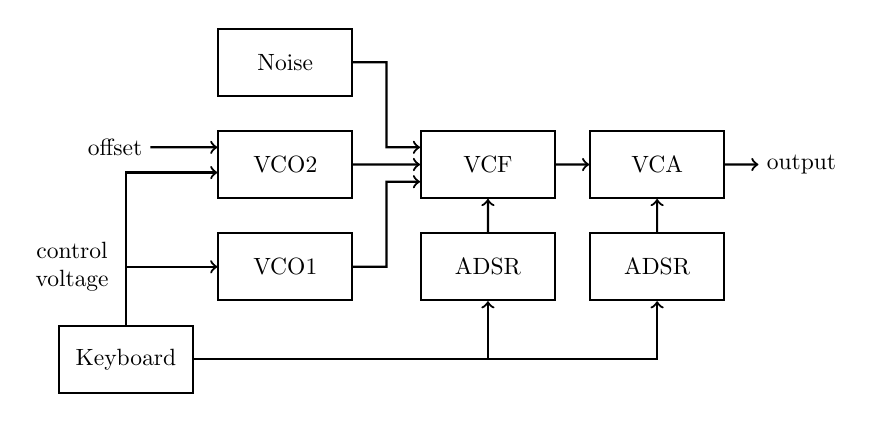
\begin{tikzpicture}[box/.style={rectangle,thick,draw=black,
minimum width=20mm, minimum height=10mm,
align=center,node distance=0.5cm},scale=0.85, transform shape]

\node at (0,0) [box] (noise) {Noise};
\node [box, below = of noise] (vco2) {VCO2};
\node [box, below = of vco2] (vco1) {VCO1};
\node [box, right = 1cm of vco2] (vcf) {VCF};
\draw [thick,->] (vco2) -- (vcf);

\coordinate (coordoffset) at ($(vco2.west)!0.5!(vco2.north west)$);

\node [left = of coordoffset](offset) {offset};
\draw [thick,->] (offset) -- (coordoffset);

\node [right = 1cm of noise] (temp1) {};

\coordinate (vcf1) at ($(vcf.west)!0.5!(vcf.north west)$);
\coordinate (vcf2) at ($(vcf.west)!0.5!(vcf.south west)$);
\coordinate (vco21) at ($(vco2.north east)!0.5!(vco2.east)$);
\coordinate (vco22) at ($(vco2.south east)!0.5!(vco2.east)$);

\node [box, right = of vcf] (vca) {VCA};
\node [box, below = of vcf] (adsr1) {ADSR};
\node [box, below = of vca] (adsr2) {ADSR};

\node [right = 0.5cm of vca] (output) {output};
\node [box, below left = 0.5cm of vco1] (keyboard) {Keyboard};

\node [left = 1.5cm of vco1,align=center](cv) {control \\ voltage };

\coordinate (noisetemp1) at ($(noise.east)!0.5!(temp1.west)$);
\coordinate (vco1adsr1) at ($(vco1.east)!0.5!(adsr1.west)$);

\coordinate (vco2vcf1) at ($(vco21)!0.5!(vcf1)$);
\coordinate (vco2vcf2) at ($(vco22)!0.5!(vcf2)$);

\draw[->,thick] (vco1.east) -- (vco1adsr1) --  (vco2vcf2) -- (vcf2);
\draw[->,thick] (noise.east) -- (noisetemp1) --  (vco2vcf1) -- (vcf1);

\draw[->,thick] (adsr1) -- (vcf);
\draw[->,thick] (adsr2) -- (vca);
\draw[->,thick] (vcf) -- (vca);
\draw[->,thick] (vca) -- (output);

\draw [thick,->] (keyboard) -| (adsr1);
\draw [thick,->] (keyboard) -| (adsr2);
\draw [thick,->] (keyboard) |- (vco1);
\draw [thick,->] (keyboard) |- (vco2.base west);
\end{tikzpicture}
\end{center}

\end{frame}


\begin{frame}
\frametitle{Fazit}

\begin{itemize}
	\item Wow\ldots
\item Riesige Bandbreite der Möglichkeiten 
\item Steile Lernkurve
\item Tolle Ergebnisse
\end{itemize}

\begin{center}

\begin{tikzpicture}
\cat[contour=black]
\end{tikzpicture}
\end{center}

\end{frame}



\end{document}



